% arara: pdflatex: { shell: yes }
\documentclass{article}
\usepackage{graphicx}
\usepackage{booktabs}
\usepackage{float}
\usepackage{hyperref}

\title{Cores Functionality}
\author{Erick Gonzalez Parada ID: 178145}
\date{\today}

\begin{document}

\maketitle

\section{Introduction}
Modern computing systems utilize multiple CPU cores to improve performance by parallelizing tasks. Multicore processors allow applications to distribute workloads across several cores, leading to improved efficiency and responsiveness. However, some applications are not optimized for multicore usage, leading to uneven resource distribution. In this report, we analyze the behavior of multicore and single-core applications through system monitoring tools to understand how they utilize processing resources \cite{theWindowsClub}.

\section{Methodology}
To evaluate CPU core utilization, we opened different applications and monitored their resource usage using the Windows Task Manager. The applications were categorized into multicore and single-core, and their CPU activity was observed and captured in screenshots.

\subsection*{Multicore}

\begin{figure}[H]
\centering
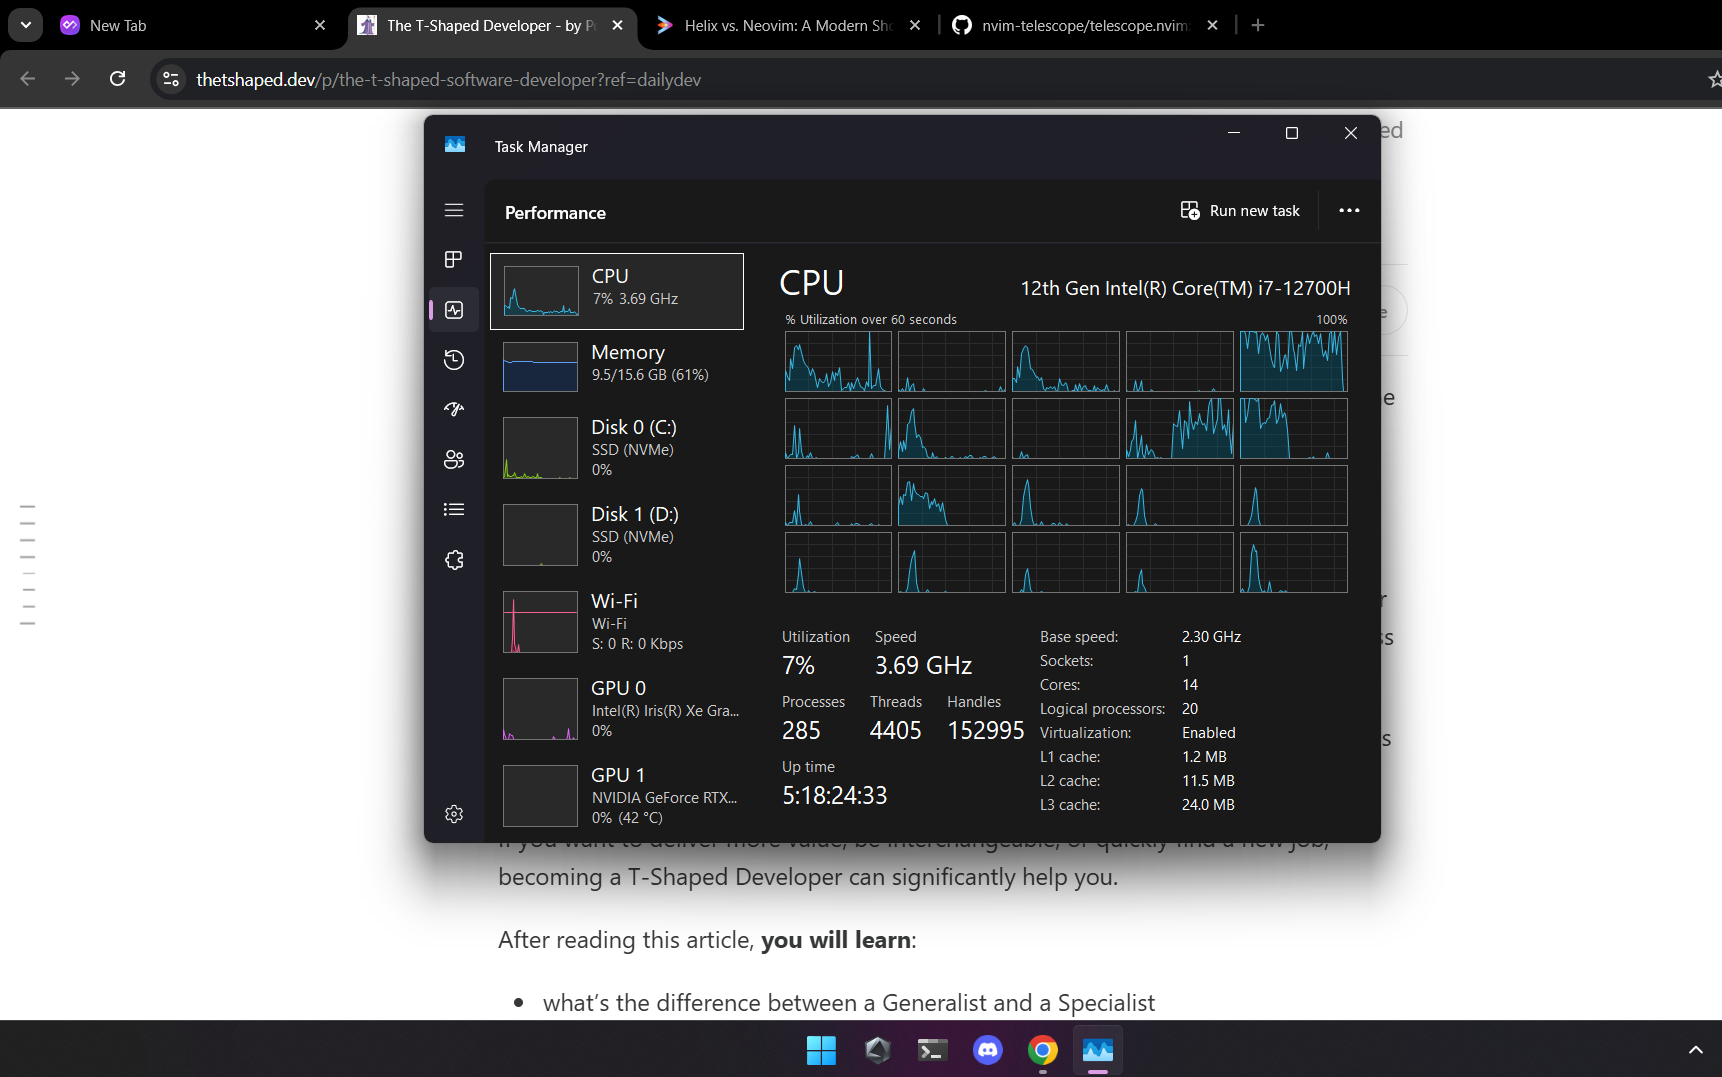
\includegraphics[width=1\textwidth]{imgs/mu1.png}
\caption{Google Chrome}
\label{fig:1}
\end{figure}
Google Chrome utilizes multiple cores to manage multiple tabs and background processes.

\begin{figure}[H]
\centering
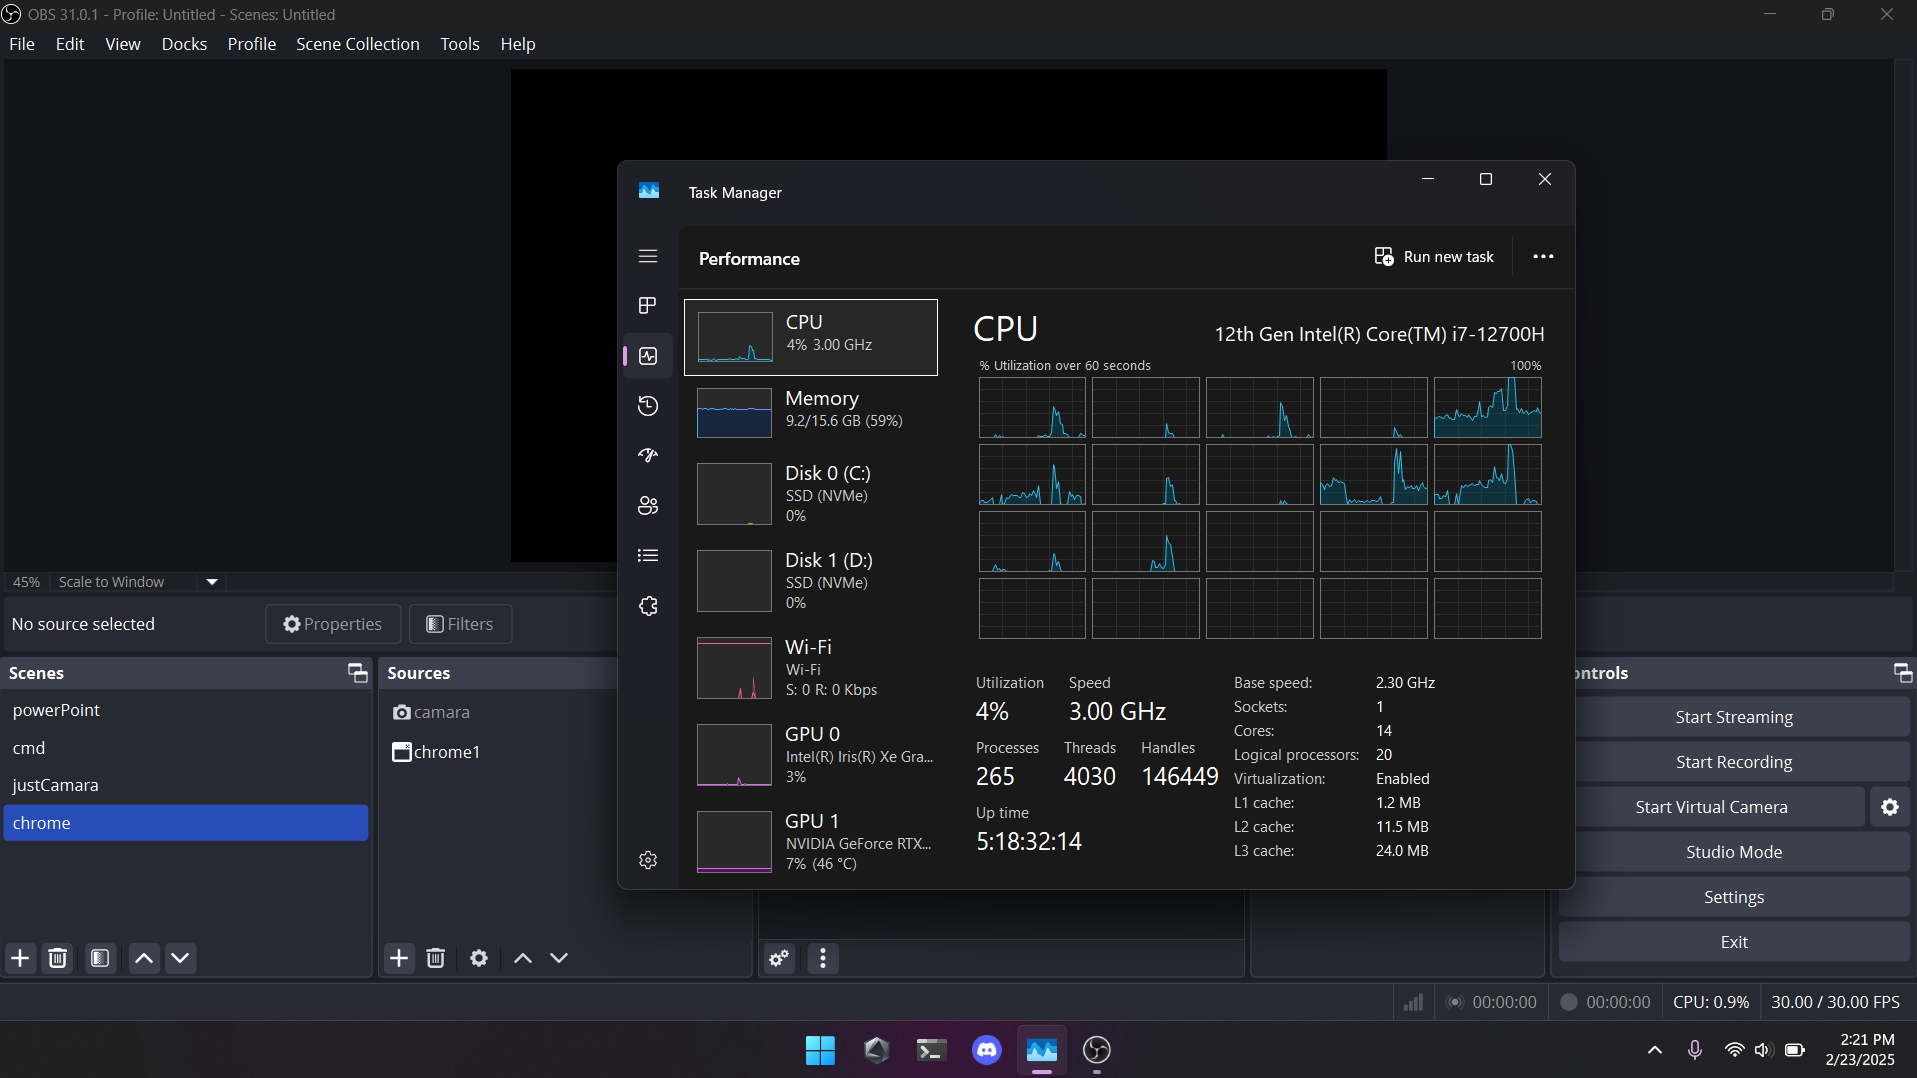
\includegraphics[width=1\textwidth]{imgs/mu2.png}
\caption{OBS software}
\label{fig:2}
\end{figure}
OBS software makes use of multiple cores for video encoding and streaming.

\begin{figure}[H]
\centering
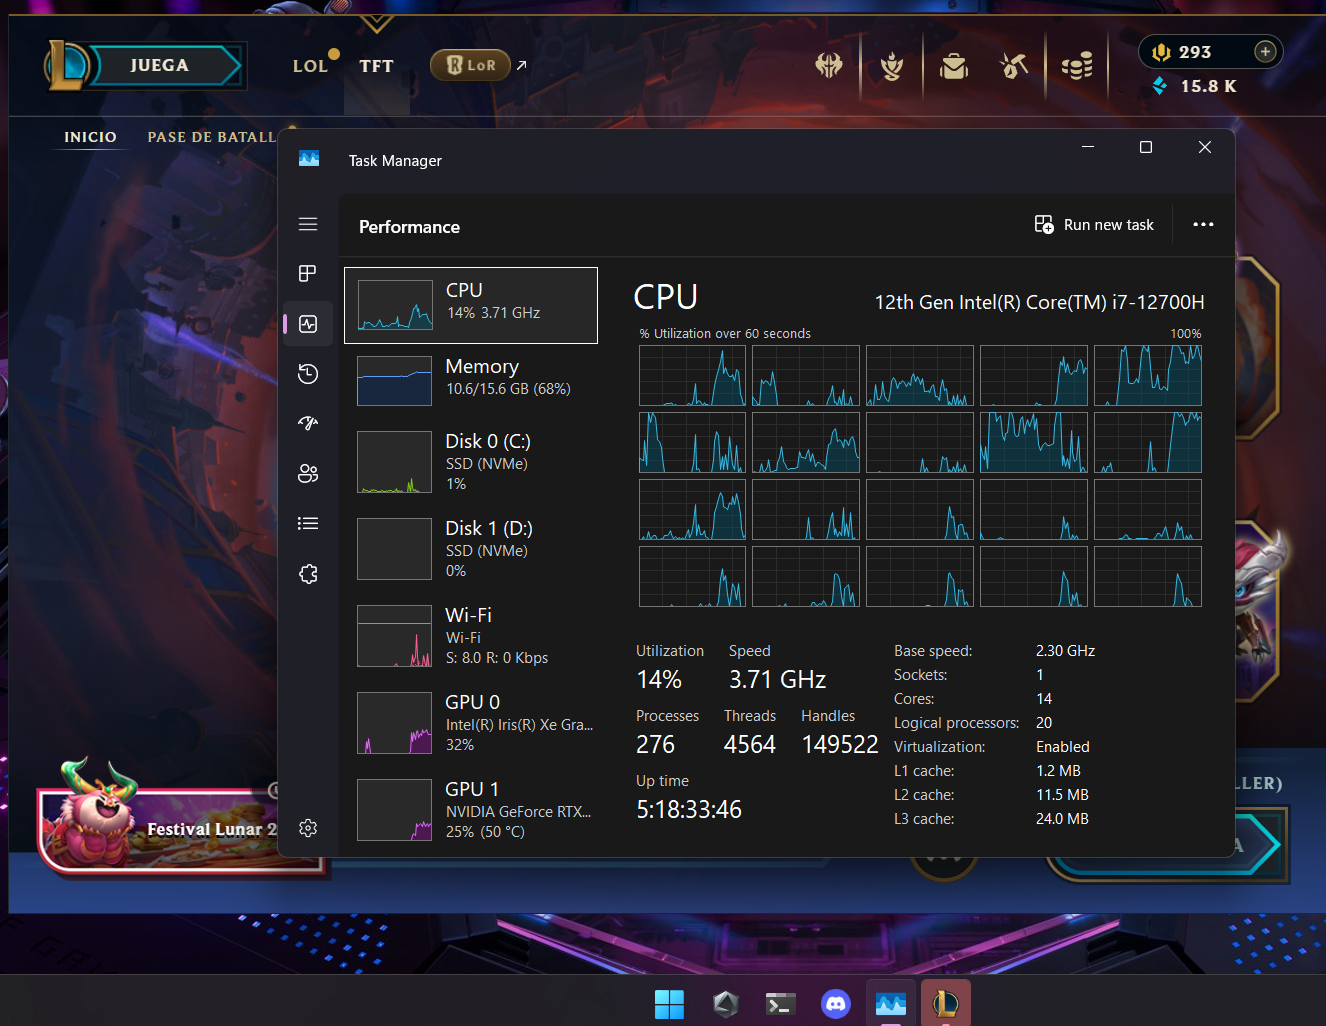
\includegraphics[width=1\textwidth]{imgs/mu3.png}
\caption{League of Legends client}
\label{fig:3}
\end{figure}
The League of Legends client employs multiple cores for rendering and network operations.

\subsection*{Singlecore}

\begin{figure}[H]
\centering
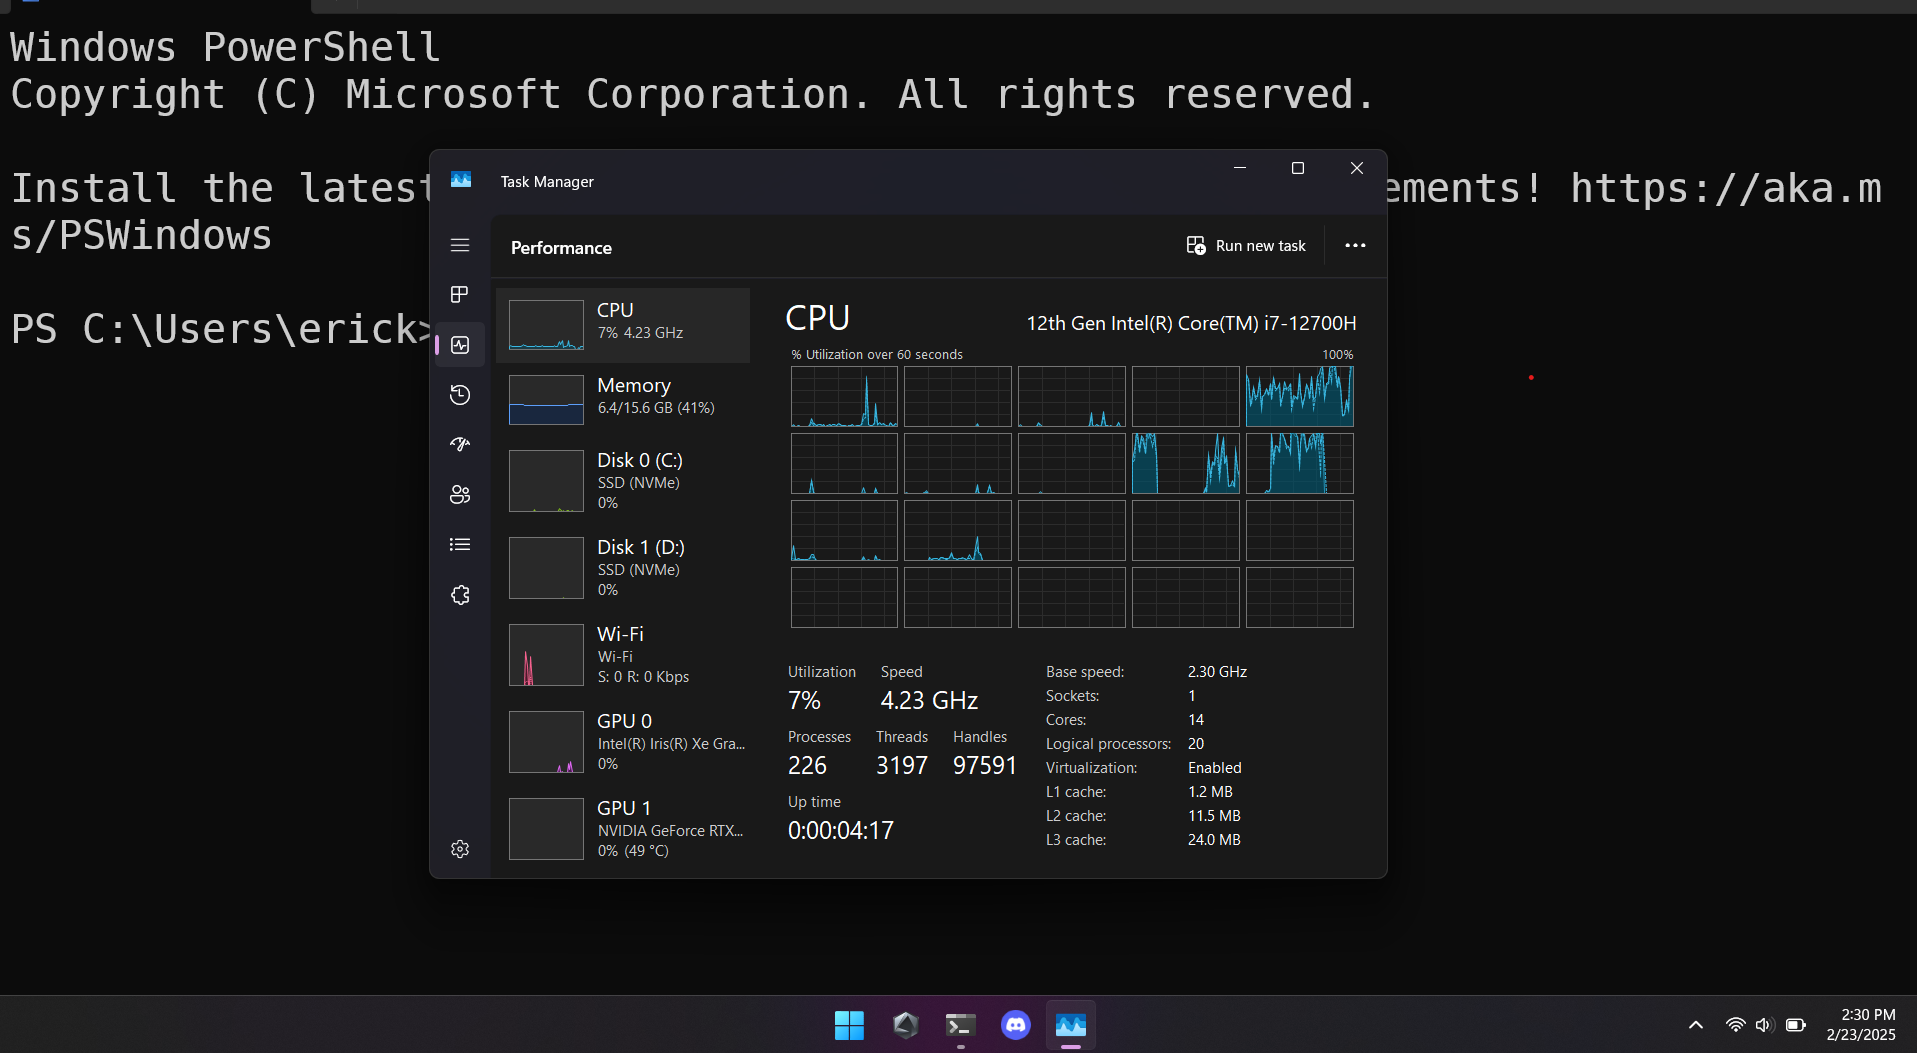
\includegraphics[width=1\textwidth]{imgs/mo1.png}
\caption{Powershell}
\label{fig:4}
\end{figure}
Powershell is expected to use a single core, but background processes may distribute the load.

\begin{figure}[H]
\centering
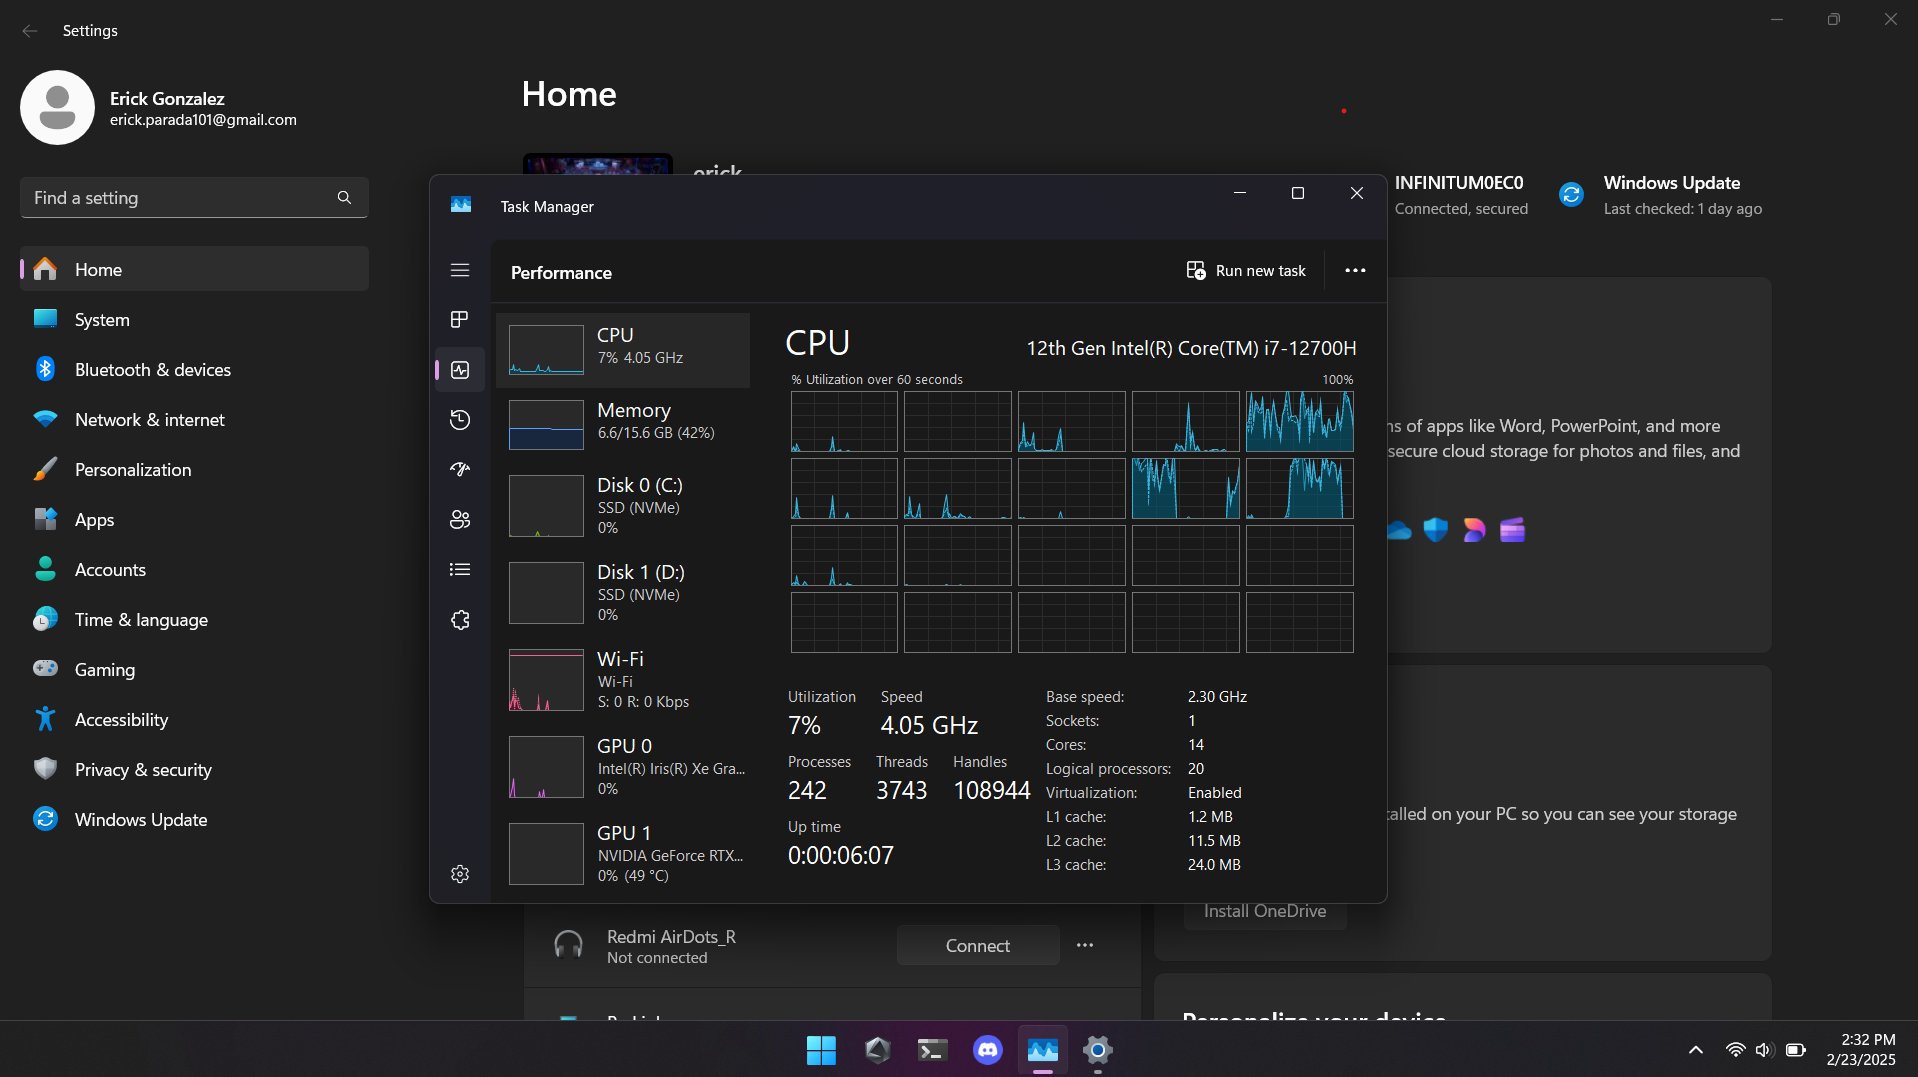
\includegraphics[width=1\textwidth]{imgs/mo2.png}
\caption{Windows Settings app}
\label{fig:5}
\end{figure}
The Windows Settings app is mostly lightweight but interacts with system services that may involve multiple cores.

\begin{figure}[H]
\centering
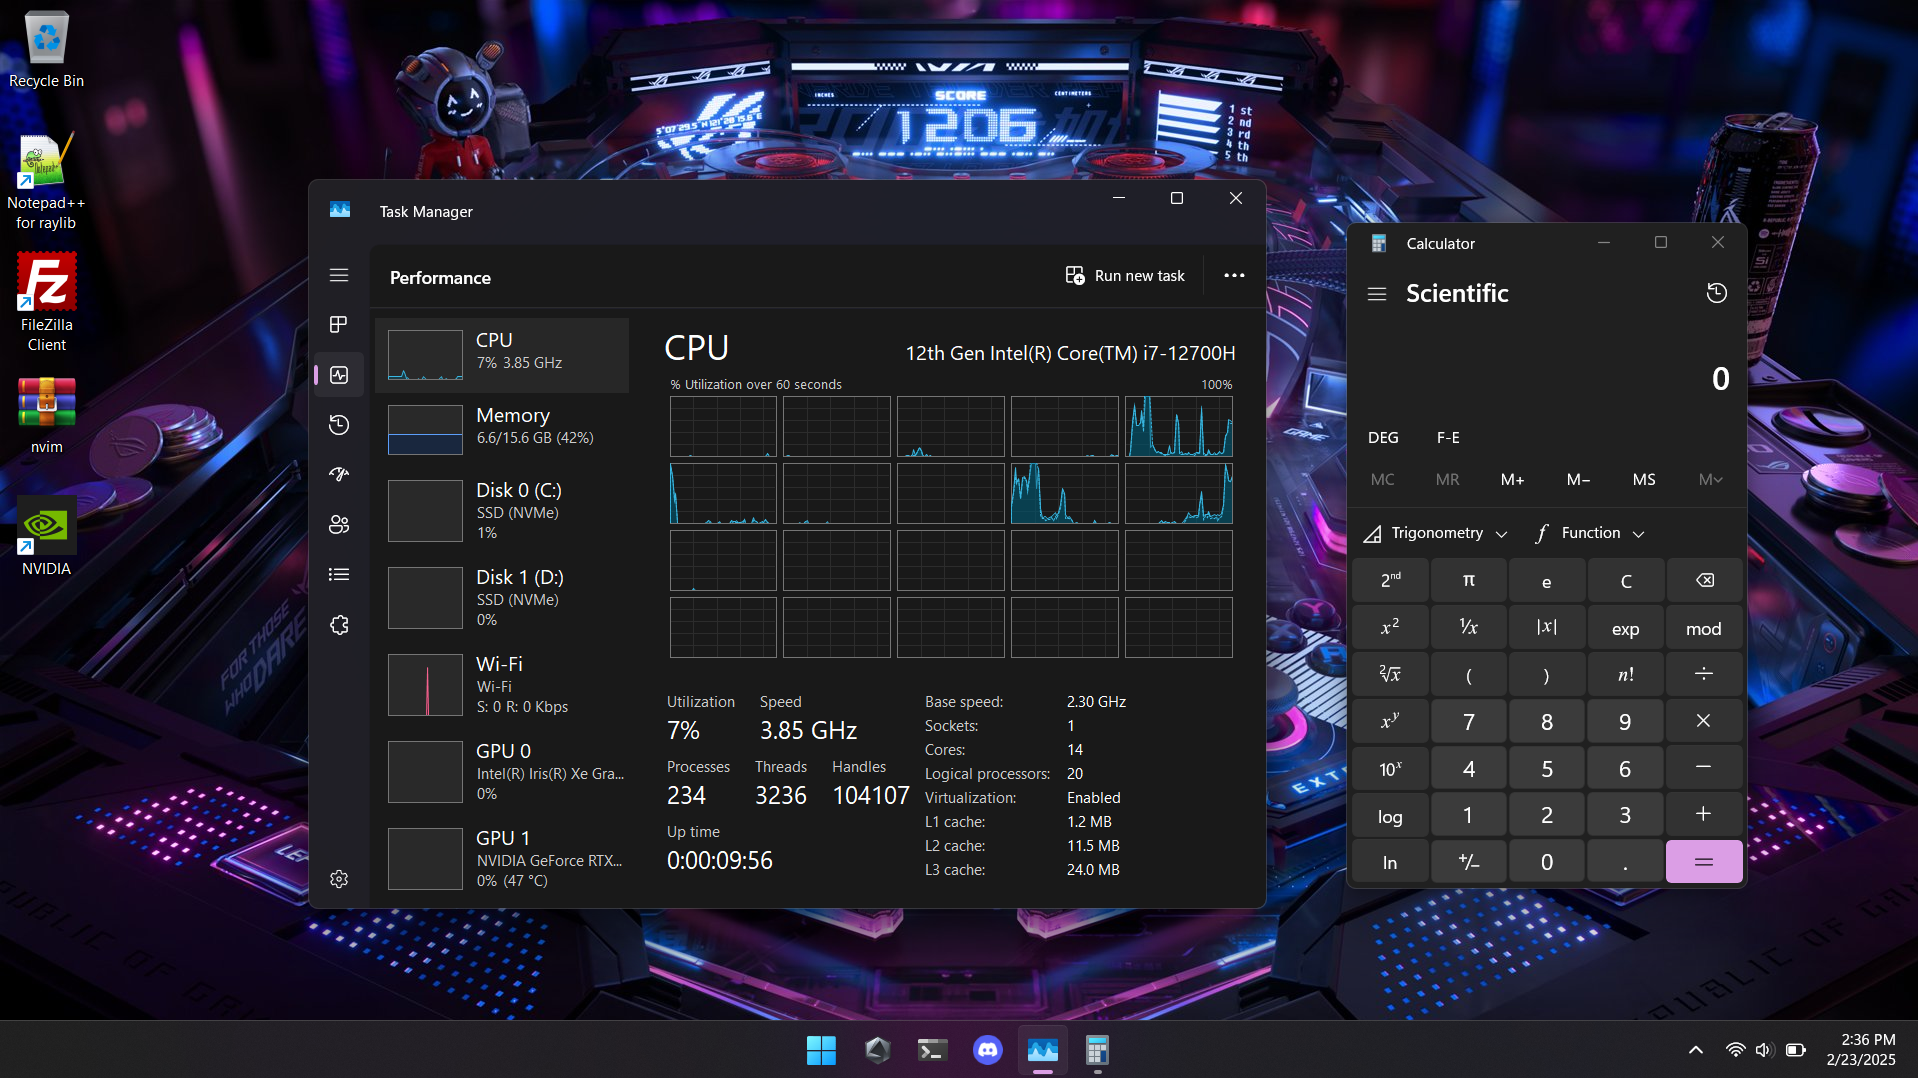
\includegraphics[width=1\textwidth]{imgs/mo3.png}
\caption{Calculator}
\label{fig:6}
\end{figure}
The Calculator is a basic application that should use minimal CPU resources but may still involve multiple threads.

\section{Analysis}
Despite being categorized as single-core applications, the observed programs did not exclusively utilize a single core. This can be attributed to modern operating system scheduling, which dynamically assigns processes across multiple cores for efficiency. Even lightweight applications have background processes and system interactions that lead to activity on more than one core.

Multicore applications, such as Google Chrome and OBS, are optimized to distribute workloads efficiently across available cores. Chrome, for example, assigns different processes to separate cores, while OBS offloads encoding tasks to multiple threads. This improves performance but also increases overall CPU utilization.

\begin{table}[H]
\centering
\begin{tabular}{ll}
\toprule
Application & Cores Used \\
\midrule
Google Chrome & Multiple \\
OBS Software & Multiple \\
League of Legends Client & Multiple \\
Powershell & Multiple \\
Windows Settings & Multiple \\
Calculator & Multiple \\
\bottomrule
\end{tabular}
\caption{Observed applications and their core usage.}
\label{tab:core_usage}
\end{table}

\section{Conclusion}
The experiment demonstrates that even applications traditionally considered single-core do not exclusively use a single processor core. This behavior is due to the operating system's task scheduling and the presence of background tasks. Applications optimized for multicore processors exhibit improved responsiveness and performance, while those that are not may experience inefficiencies when handling complex tasks. Understanding core utilization helps in evaluating system performance and optimizing workload distribution.

\begin{thebibliography}{9}
\bibitem{theWindowsClub}
What are CPU cores? How many CPU cores do I need? (2021, May 28). The Windows Club; TheWindowsClub. \url{https://www.thewindowsclub.com/what-are-cpu-cores}
\end{thebibliography}

\end{document}

